\documentclass[tikz,border=8pt]{standalone}
\usepackage{amsmath}
\usetikzlibrary{arrows.meta,positioning,fit,calc}
\definecolor{blue}{HTML}{0072B2}\definecolor{orange}{HTML}{E69F00}
\definecolor{green}{HTML}{009E73}\definecolor{ink}{HTML}{172033}
\definecolor{pale}{HTML}{F2F4F7}\definecolor{muted}{HTML}{667085}
\begin{document}
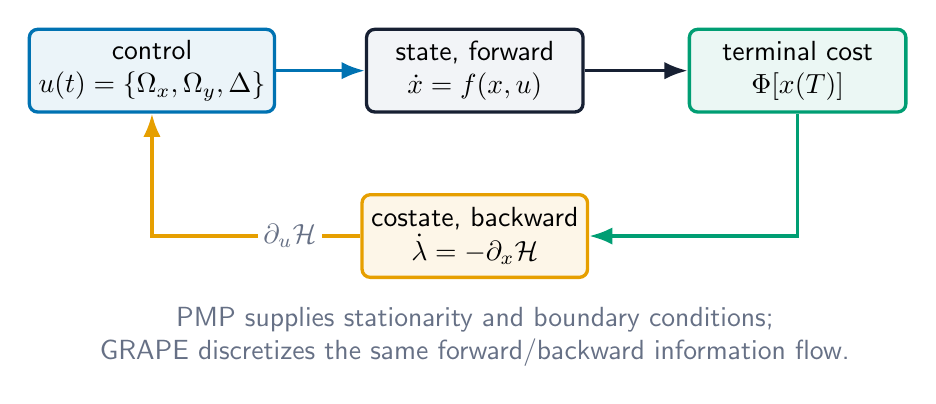
\begin{tikzpicture}[font=\sffamily,>=Latex,
box/.style={rounded corners=3pt,minimum width=2.75cm,minimum height=1.05cm,align=center,very thick}]
  \node[box,draw=blue,fill=blue!8] (control) at (0,2.3) {control\\$u(t)=\{\Omega_x,\Omega_y,\Delta\}$};
  \node[box,draw=ink,fill=pale] (forward) at (4.1,2.3) {state, forward\\$\dot x=f(x,u)$};
  \node[box,draw=green,fill=green!8] (cost) at (8.2,2.3) {terminal cost\\$\Phi[x(T)]$};
  \node[box,draw=orange,fill=orange!9] (costate) at (4.1,.2) {costate, backward\\$\dot\lambda=-\partial_x\mathcal H$};
  \draw[->,very thick,blue] (control) -- (forward);
  \draw[->,very thick,ink] (forward) -- (cost);
  \draw[->,very thick,green] (cost) |- (costate);
  \draw[->,very thick,orange] (costate) -| (control);
  \node[muted,fill=white,inner sep=2pt] at (1.75,.2) {$\partial_u\mathcal H$};
  \node[align=center,muted] at (4.1,-1.08) {PMP supplies stationarity and boundary conditions;\\GRAPE discretizes the same forward/backward information flow.};
\end{tikzpicture}
\end{document}
